\section{Case studies}
\label{sec:cases}
We ran a fixed panel of 156 simulation records covering chemical inputs, sensory combinations, and experience-dependent responses. Each condition used seeds 11, 23, and 47, with the same probe inputs across memory histories. The records contain the actual neural inputs, sparse activity, population and motor summaries, and memory before and after each step. The numerical experiments used explicit stimulus recipes, with the planner, narrator, and soft-token reader disabled. This separates the model's response from errors introduced by language interpretation. The seeds characterize stochastic variability in one assembled model.

\subsection{Chemical inputs produce repeatable, differentiated KC codes}
The chemical panel comprised ethyl acetate, methyl acetate, 1-hexanol, Z3-hexenol, acetic acid, and pyrrolidine. It was fixed using the existing chemical list and DoOR coverage/similarity, before examining the new neural outputs. Depending on the chemical, measurements covered 27--45 of the 53 modeled glomeruli; 7--24 glomeruli remained above the drive threshold. Each chemical was presented for 250 ms at the default response-to-rate conversion.

The fraction of Kenyon cells active during a probe ranged from 1.64\% to 12.65\%. We represent a code by the set of KCs that fired and compare two codes using Jaccard overlap, $|A\cap B|/|A\cup B|$. Mean within-chemical overlap across pairs of seeds ranged from 0.725 to 0.915 (Figure~\ref{fig:olfaction}a). Ethyl and methyl acetate had high receptor-profile similarity and mean KC overlap of 0.756; ethyl acetate and pyrrolidine had KC overlap of 0.002. Across the 15 chemical pairs, receptor-profile cosine similarity and mean KC overlap had a descriptive Pearson correlation of 0.692 (Figure~\ref{fig:olfaction}b). The relationship shows how similarity propagates through this selected panel; the pairs share chemicals and are not 15 independent biological observations.

\begin{figure}[t]
\centering
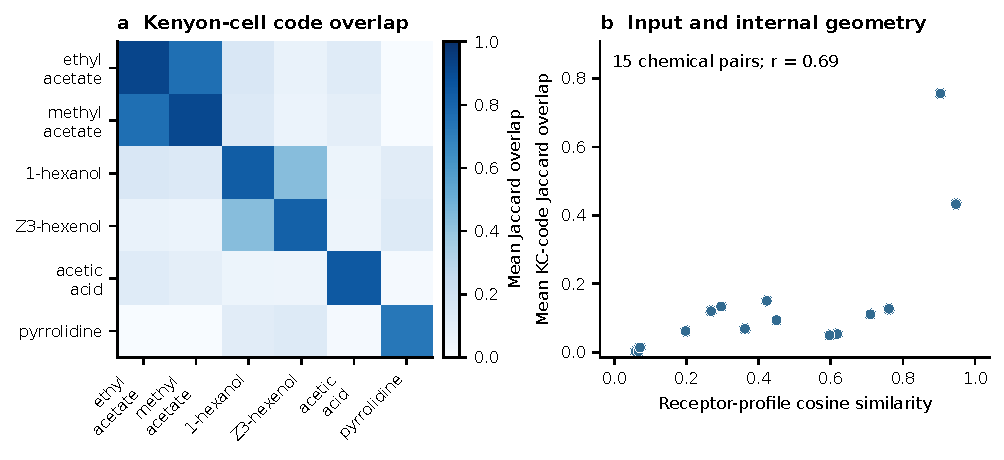
\includegraphics[width=\linewidth]{figures/fig2_olfaction.pdf}
\caption{Chemical inputs produce repeatable and differentiated KC activity. \textbf{a}, Mean Jaccard overlap between active-KC sets. Diagonal entries compare the three distinct pairs of seeds for the same chemical; off-diagonal entries average all nine combinations of seeds for two chemicals. \textbf{b}, Receptor-profile cosine similarity, computed only over jointly measured glomeruli, versus mean KC overlap for all 15 chemical pairs. The correlation is descriptive for the fixed six-chemical panel.}
\label{fig:olfaction}
\end{figure}

\subsection{Sensory combinations reach distinct motor-output channels}
The sensory panel comprised zero-rate input, sugar, bitter, sugar plus bitter, antennal touch, and looming-pathway stimulation. Sugar, bitter, and touch used 150 Hz input; looming used 200 Hz. All brain probes lasted 250 ms. We report the maximum firing rate within each annotated output group, averaged across the three seeds.

Adding bitter to sugar reduced the proboscis-output peak from 73.3 to 14.7 Hz, while the zero-rate and bitter-alone conditions produced no proboscis output (Figure~\ref{fig:sensorimotor}a). Looming produced a 240.0 Hz peak in the escape group, and antennal touch produced a 62.7 Hz peak in the antennal-grooming group. These are model-output channels grounded in circuit annotations; the experiment measures neural activity, not executed movement.

For the VNC bridge, we drove the giant-fiber type DNp01 at 240 Hz for 300 ms. TTMn reached 56.7--60.0 Hz across the three seeds. Five other descending-neuron pairs, selected with a fixed random seed and excluding DNp01, produced no TTMn spikes in any of their 15 probes (Figure~\ref{fig:sensorimotor}b). This control characterizes the tested descending-to-motor route. The general sensory panel additionally records the VNC response to 200 ms of transferred descending rates.

\begin{figure}[t]
\centering
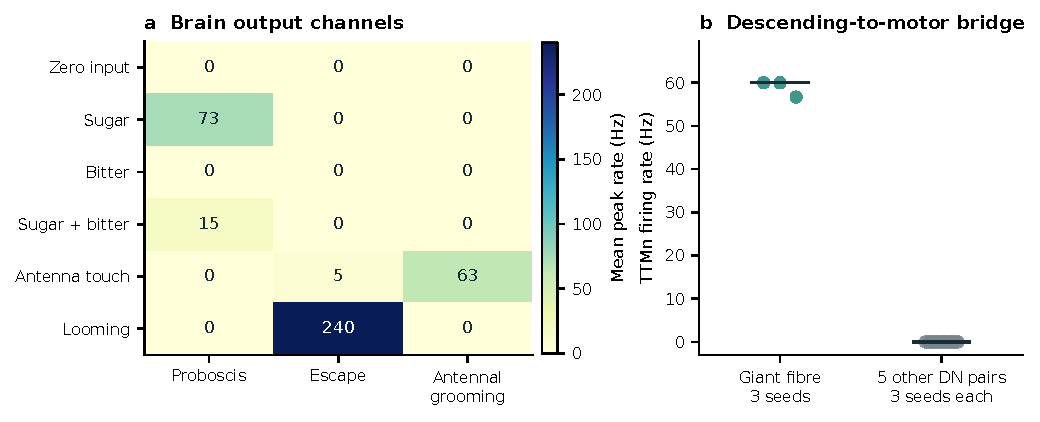
\includegraphics[width=\linewidth]{figures/fig3_sensorimotor.pdf}
\caption{Sensory inputs reach distinct neural output channels. \textbf{a}, Mean across three seeds of the maximum rate within each annotated brain-output group. Sugar plus bitter suppresses the proboscis-output peak relative to sugar alone. \textbf{b}, TTMn rates during giant-fiber stimulation and the five fixed comparison pairs of descending drivers; each dot is one simulation and horizontal marks indicate medians. The bridge predicts motor-neuron activity, without a biomechanical body.}
\label{fig:sensorimotor}
\end{figure}

\subsection{Experience changes odor responses and survives state restoration}
We tested ethyl acetate and pyrrolidine in two independent histories. History A paired ethyl acetate with PAM reward drive and pyrrolidine with PPL1 punishment drive; history B reversed these assignments. Each odor received three training presentations, with reinforcement at 60 Hz. A third history separated each odor pulse from its reinforcement pulse and reset membrane dynamics between pulses. The batch experiment applied the plasticity update after every training pulse, including isolated ones. Ordinary \texttt{FlyChat} interactions instead call the update only for an explicit reward or punishment request paired with an odor. The batch policy is part of the evaluated protocol.

We summarize MBON output with the implemented valence index $(R_{\mathrm{approach}}-R_{\mathrm{avoid}})/(R_{\mathrm{approach}}+R_{\mathrm{avoid}}+1)$, where the two rates sum activity in predefined MBON groups. Positive and negative values indicate the model's approach- and avoidance-associated output balance. Ethyl acetate shifted from a mean naive index of 0.19 to 0.67 after reward pairing and to $-0.43$ after punishment pairing (Figure~\ref{fig:memory}a). Pyrrolidine shifted from 0.49 to $-0.80$ after punishment pairing, while reward pairing did not consistently increase its index (Figure~\ref{fig:memory}b). The pyrrolidine index is supported by only 1--21 contributing spikes in the 250-ms probes (Table~\ref{tab:memory-counts}); its reward-response variation should be read at this finite-window scale. Loading the saved history-A state reproduced the complete spike-count vector exactly for all six matched odor probes.

The unpaired history exposed an additional consequence of the implemented rule. Ethyl acetate shifted from 0.19 to $-0.04$ even though external odor and reinforcement pulses were separated. Each of its nine odor-only training pulses recruited 13--17 dopamine neurons and weakened 830--2,393 synapses. The 18 isolated reinforcement pulses had no KC activity and no weight updates. Thus, externally unpaired stimulation did not remove internal KC--DAN coactivation. The observed history dependence is persistent and traceable, but cannot be described as learning restricted to externally paired events. Pyrrolidine's unpaired probe index was unchanged from its matched naive value for each seed.

\begin{figure}[t]
\centering
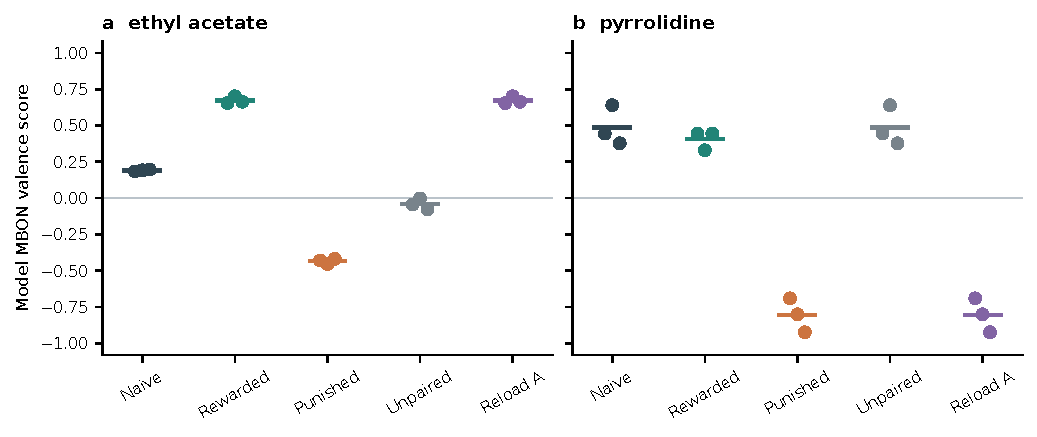
\includegraphics[width=\linewidth]{figures/fig4_memory.pdf}
\caption{The same chemical input elicits different MBON outputs after different experience. Dots show the three matched probe seeds; horizontal marks show means. Rewarded and punished conditions come from separate histories, with opposite assignments for the two chemicals. Reload A restores the ethyl-acetate-reward/pyrrolidine-punishment history and reproduces all six spike-count vectors exactly. Ethyl acetate also changes under the externally unpaired protocol, where its odor-only pulses recruit dopamine neurons. This control limits a paired-only learning interpretation.}
\label{fig:memory}
\end{figure}

\subsection{Recorded interactions connect language to numerical evidence}
We completed a fixed panel of 18 interactions: 12 natural-language requests and six controlled memory queries, using 39 live LLM calls. The natural-language cases exercised the planner with duration fixed to 250 ms. For the memory queries, the original planner output was saved, then the chemical input and loaded memory state were fixed by the protocol. These six queries test interpretation of matched states, rather than planner accuracy. Independent checks of their saved arrays confirmed exact agreement with the corresponding case-C inputs, memory, and spike-count vectors for all six probes.

The interface preserved an explicit zero-rate request and the specified 400 Hz sound frequency and 0.5 amplitude. An apple request was resolved to a disclosed hexyl-acetate proxy, making the connection from an everyday description to an available chemical explicit. The two sugar phrasings, however, selected different input implementations, and the two looming phrasings used different rates; these examples do not establish identical-input invariance to paraphrasing.

For identical ethyl-acetate probes, the narrator described the positive learned shift in history A and the negative shift in history B (Table~\ref{tab:dialogue}). Across the six controlled memory queries, its statements about the direction or absence of a learned index change agreed with the records. The narrator received explicit valence summaries, so these explanations characterize record-informed narration, separately from the neural-state-only reader.
\begin{table}[t]
\caption{Short translated excerpts connect two memory states to the same query and preserve a concrete error from the fixed panel. The memory query was ``Present ethyl acetate, without reinforcement.'' Values are the recorded model indices for seed 11; the narrator was supplied these summaries. Ellipses mark omitted text; complete Russian replies are retained in the artifact.}
\label{tab:dialogue}
\small
\begin{tabularx}{\linewidth}{@{}p{0.18\linewidth}p{0.16\linewidth}X@{}}
\toprule
Condition & Recorded value & Translated narrator excerpt \\
\midrule
Ethyl acetate, history A & $+0.65$ (naive $+0.18$) & ``The naive estimate was weak (+0.18), but with memory it jumped to +0.65.'' \\
Ethyl acetate, history B & $-0.43$ (naive $+0.18$) & ``Naive attraction would be weakly positive \ldots\ the smell pulls me away.'' \\
Sugar paraphrase & Right 100 Hz; left 68 Hz & ``The left CB0701 motor neuron fires at about 100 Hz, the right at 68 Hz.'' This reverses the recorded sides. \\
\bottomrule
\end{tabularx}
\end{table}


We audited the 18 replies against their saved traces using an AI-assisted, independently checked record review for author inspection. The post-hoc categories identified two replies with clear trace contradictions: swapped left/right motor rates, and a weak-odor assertion when the resolver was unmapped and no odor input was delivered. Four replies contained explanations not established by the panel, three described physical effects beyond the simulated neural output, and three blurred zero learned change with neutral absolute valence. Categories may overlap. Every reply contained at least one checked factual anchor, which does not certify its remaining claims. These counts describe this fixed panel and its audit rubric, not a blinded human evaluation or an overall faithfulness percentage.

Finally, replaying the recorded natural-language sugar case required no LLM calls and reproduced sparse spike counts, spike times within $10^{-9}$ s, VNC driver rates, and VNC motor rates. Accepted inputs and state can therefore be replayed separately from the language calls that produced or explained them.
